% Figures/cake-paths.tex
% Optimal paths of the continuous-time cake-eating problem, Proposition
% \ref{prop:ct-cake} of Chapter \ref{ch:continuoustime}:
% k^*(t)=k_0e^{-rt} and c^*(t)=rk_0e^{-rt}, drawn for r=0.4 and k_0=1.
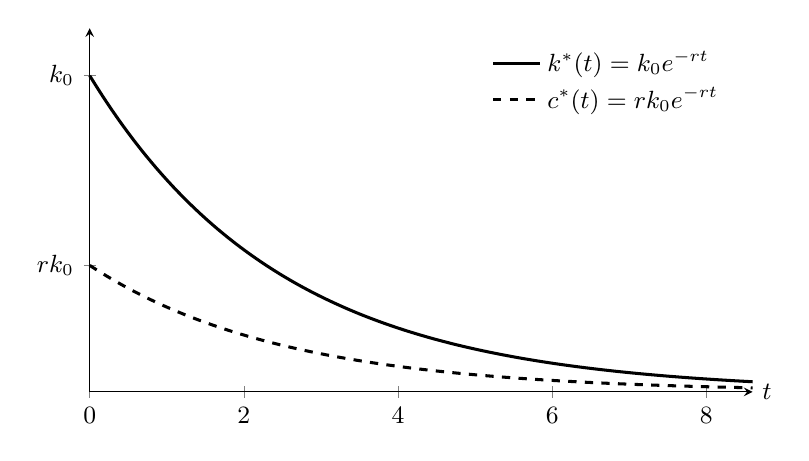
\begin{tikzpicture}
	\begin{axis}[
			width=10cm, height=6.2cm,
			axis lines=left,
			xlabel={$t$},
			every axis x label/.style={at={(current axis.right of origin)},anchor=west},
			xmin=0, xmax=8.6, ymin=0, ymax=1.15,
			xtick={0,2,4,6,8},
			ytick={0.4,1}, yticklabels={$rk_0$,$k_0$},
			tick label style={font=\small},
			label style={font=\small},
			legend cell align=left,
			legend style={draw=none, fill=none, font=\small,
					at={(0.97,0.97)}, anchor=north east},
			clip=false,
		]
		\addplot[line width=1.1pt, domain=0:8.6, samples=120] {exp(-0.4*x)};
		\addlegendentry{$k^{\ast}(t)=k_0e^{-rt}$}

		\addplot[line width=1.1pt, dashed, domain=0:8.6, samples=120]
		{0.4*exp(-0.4*x)};
		\addlegendentry{$c^{\ast}(t)=rk_0e^{-rt}$}
	\end{axis}
\end{tikzpicture}
